\documentclass[a4paper,12pt]{article}
\usepackage[utf8]{inputenc}
\usepackage[german]{babel}
\usepackage{amsmath}
\usepackage{amssymb}
\usepackage{amsthm}
\usepackage{geometry}
\usepackage{graphicx}
\usepackage[hidelinks]{hyperref}
\usepackage{listings}
\usepackage{xcolor}
\usepackage{enumitem}
\usepackage{booktabs}
\usepackage{array}
\usepackage{caption}
\usepackage{subcaption}

\geometry{margin=2.5cm}

\theoremstyle{definition}
\newtheorem{definition}{Definition}
\newtheorem{beispiel}{Beispiel}
\newtheorem{satz}{Satz}
\newtheorem{lemma}{Lemma}
\newtheorem{bemerkung}{Bemerkung}
\newtheorem{korollar}{Korollar}
\newtheorem{proposition}{Proposition}

\setlist[itemize,1]{label=--}

% ---------- Farben ----------
\definecolor{mainblue}{RGB}{25, 70, 140}
\definecolor{accentred}{RGB}{180, 50, 30}
\definecolor{lightgray}{RGB}{245, 245, 248}
\definecolor{darkgray}{RGB}{60, 60, 70}
\definecolor{darkgreen}{RGB}{30, 100, 50}

\hypersetup{
	colorlinks=true,
	linkcolor=mainblue,
	citecolor=accentred,
	urlcolor=mainblue
}

\lstset{
	basicstyle=\ttfamily\small,
	keywordstyle=\color{blue},
	commentstyle=\color{gray},
	stringstyle=\color{red},
	numbers=left,
	numberstyle=\tiny,
	breaklines=true,
	frame=single,
}

\title{\textbf{Lernbasiertes Autonomes Netzwerkmanagement\\
in Heterogenen Mobilfunknetzen}\\[0.5em]
\large Formale Analyse, Optimierungsmodelle und Multi-Agent-Erweiterungen
auf Basis von Reinforcement Learning}
\author{Stephan Epp\\
\small Universit\"at Bielefeld\\
\small \texttt{stephan.epp@uni-bielefeld.de}}
\date{3. Juni 2026}

\begin{document}

\maketitle

\begin{abstract}
Heterogene Mobilfunknetze (HetNets) stehen vor der Herausforderung, dynamische
Benutzergerät-Lebenszyklen, variierende Lastverteilungen und hohe Energieeffizienzanforderungen
gleichzeitig zu beherrschen. In dieser Arbeit analysieren wir das von Illian~\cite{illian2026}
vorgestellte lernbasierte autonome Netzwerkmanagementsystem \emph{CellPilot} formal und
exhaustiv. Wir modellieren die Leerlauf-Selektion von Mobilfunkzellen als partiell
beobachtbares Markov-Entscheidungsprozess (POMDP) und zeigen, dass der REINFORCE-Algorithmus
mit Reward-Shaping-Baselines zur Policy-Konvergenz führt. Des Weiteren formulieren wir die
Bandwechsel-Energieoptimierung im Verbindungsmodus als gemischt-ganzzahliges konvexes
Optimierungsproblem (MIQCP) und beweisen die Existenz einer eindeutigen optimalen Lösung
unter gegebenen Kapazitätsnebenbedingungen. Alle Ergebnisse werden analytisch hergeleitet,
formal bewiesen und durch umfangreiche Simulationen mit synthetischen sowie realen
3GPP-konformen Leistungsmodellen validiert. Der Ausblick beschreibt detailliert die
Erweiterung auf Multi-Agent-RL-Architekturen sowie die Integration in 5G/6G-Netzwerkschichten.
\end{abstract}

\tableofcontents
\newpage

%==========================================================
\section{Einf\"uhrung}
%==========================================================

Moderne Mobilfunknetze entwickeln sich hin zu heterogenen Architekturen (HetNets), in
denen Makrozellen, Kleinzellen (Small Cells) und millimeterwellenbasierte Zugangsknoten
koexistieren. Gleichzeitig w\"achst die Anzahl der User Equipment (UE) rapide, und die
Anforderungen an Energieeffizienz -- sowohl seitens des Netzbetreibers als auch im Hinblick
auf die Akkulaufzeit der Endgeräte -- steigen stetig. Klassische regelbasierte Steuerungslogik
ist den komplexen, nichtstation\"aren Bedingungen dieser Netze nicht gewachsen.

Reinforcement Learning (RL) bietet eine elegante Alternative: Ein Agent lernt eine
Netzwerksteuerungs-Policy durch wiederholte Interaktion mit der Umgebung und optimiert dabei
eine langfristige Reward-Funktion ohne explizit modellierte Systemdynamik. Die vorliegende
Arbeit untersucht das von Illian~\cite{illian2026} vorgestellte System \emph{CellPilot}
wissenschaftlich und ergänzt es durch formale mathematische Beweise, ausführliche
Herleitung der Optimierungsprobleme sowie extensive Simulationsresultate.

\subsection{Beitrag dieser Arbeit}

Diese Arbeit leistet folgende Beiträge:
\begin{itemize}
  \item Formale POMDP-Modellierung des Leerlauf-Zellselektionsproblems (Abschnitt~\ref{sec:pomdp})
  \item Beweis der Policy-Konvergenz des REINFORCE-Algorithmus mit Baselines (Abschnitt~\ref{sec:reinforce})
  \item MIQCP-Formulierung der Bandwechsel-Energieoptimierung und Beweis der Optimalität (Abschnitt~\ref{sec:miqcp})
  \item Analytische Herleitung und Validierung des 3GPP-konformen UE-Leistungsmodells (Abschnitt~\ref{sec:power})
  \item Simulative Validierung aller Ergebnisse mit matplotlib-Visualisierungen (Abschnitt~\ref{sec:experimente})
  \item Detaillierter Ausblick auf Multi-Agent-RL-Erweiterungen und 5G/6G-Integration (Abschnitt~\ref{sec:ausblick})
\end{itemize}

\subsection{Verwandte Arbeiten}

Lernbasiertes Netzwerkmanagement wurde in den letzten Jahren intensiv untersucht.
Deep-Q-Network-basierte (DQN) Ansätze für Handover-Entscheidungen wurden in~\cite{fehske2011}
und~\cite{zhang2019} beschrieben. POMDP-Formulierungen für HetNet-Ressourcenzuweisung finden
sich in~\cite{li2020}. Die Verwendung des REINFORCE-Algorithmus f\"ur Policy-Gradient-Optimierung
in Telekommunikationsnetzen ist in~\cite{sutton2018} grundlegend beschrieben. Das Subgraph-basierte
Optimierungsframework von Epp~\cite{epp2026sub} liefert dabei allgemeine Methoden zur strukturellen
Graphoptimierung, die direkt auf Netztopologien übertragbar sind.

%==========================================================
\section{Grundlagen}
%==========================================================

\subsection{Heterogene Mobilfunknetze}

\begin{definition}[Heterogenes Netzwerk]
  Ein heterogenes Mobilfunknetz (HetNet) ist ein System
  $\mathcal{N} = (\mathcal{B}, \mathcal{U}, \mathcal{L})$,
  wobei $\mathcal{B} = \{b_1, \ldots, b_M\}$ die Menge der Basisstationen,
  $\mathcal{U} = \{u_1, \ldots, u_K\}$ die Menge der User Equipment und
  $\mathcal{L} \subseteq \mathcal{B} \times \mathcal{U}$ die zulässigen
  Verbindungsrelationen bezeichnet.
\end{definition}

\begin{definition}[Leerlaufmodus und Verbindungsmodus]
  Ein UE $u_k \in \mathcal{U}$ befindet sich im \emph{Leerlaufmodus} (idle mode),
  wenn keine aktive Datenverbindung besteht. Es befindet sich im \emph{Verbindungsmodus}
  (connected mode), wenn eine aktive Datenübertragung stattfindet. Der Übergang zwischen
  beiden Modi erfolgt durch ein \emph{Handover}-Ereignis.
\end{definition}

\begin{definition}[Referenzsignalempfangspegel -- RSRP]
  Der RSRP (Reference Signal Received Power) eines UE $u_k$ zur Basisstation $b_j$ ist
  definiert als:
  \[
    \mathrm{RSRP}_{k,j} = P_j - \mathrm{PL}_{k,j} - X_{\sigma}
  \]
  wobei $P_j$ die Sendeleistung, $\mathrm{PL}_{k,j}$ den Pfadverlust und
  $X_{\sigma} \sim \mathcal{N}(0, \sigma^2)$ das Log-Normal-Shadowing bezeichnet.
\end{definition}

\subsection{Markov-Entscheidungsprozesse}

\begin{definition}[MDP]
  Ein Markov-Entscheidungsprozess (MDP) ist ein Tupel
  $\mathcal{M} = (\mathcal{S}, \mathcal{A}, P, R, \gamma)$, wobei:
  \begin{itemize}
    \item $\mathcal{S}$ die Zustandsmenge,
    \item $\mathcal{A}$ die Aktionsmenge,
    \item $P: \mathcal{S} \times \mathcal{A} \times \mathcal{S} \to [0,1]$ die Übergangswahrscheinlichkeit,
    \item $R: \mathcal{S} \times \mathcal{A} \to \mathbb{R}$ die Reward-Funktion und
    \item $\gamma \in [0,1)$ den Diskontfaktor bezeichnet.
  \end{itemize}
\end{definition}

\begin{definition}[POMDP]
  Ein partiell beobachtbares MDP (POMDP) erweitert das MDP um einen
  Beobachtungsraum $\mathcal{O}$ und eine Beobachtungswahrscheinlichkeit
  $\Omega: \mathcal{S} \times \mathcal{A} \times \mathcal{O} \to [0,1]$:
  \[
    \mathcal{P} = (\mathcal{S}, \mathcal{A}, P, R, \mathcal{O}, \Omega, \gamma).
  \]
  Der Agent beobachtet nicht direkt $s \in \mathcal{S}$, sondern nur
  $o \in \mathcal{O}$ mit $P(o \mid s, a) = \Omega(s, a, o)$.
\end{definition}

\subsection{Policy-Gradient-Methoden}

\begin{definition}[Stochastische Policy]
  Eine stochastische Policy $\pi_\theta: \mathcal{S} \times \mathcal{A} \to [0,1]$
  mit Parametervektor $\theta \in \mathbb{R}^d$ gibt für jeden Zustand $s$
  eine Wahrscheinlichkeitsverteilung über Aktionen an:
  $\pi_\theta(a \mid s) \geq 0$ und $\sum_{a \in \mathcal{A}} \pi_\theta(a \mid s) = 1$.
\end{definition}

\begin{definition}[Erwarteter Return]
  Der erwartete diskontierte Return einer Policy $\pi_\theta$ ist:
  \[
    J(\theta) = \mathbb{E}_{\tau \sim \pi_\theta}\!\left[\sum_{t=0}^{T} \gamma^t R(s_t, a_t)\right]
  \]
  wobei $\tau = (s_0, a_0, r_0, s_1, \ldots)$ eine Trajektorie bezeichnet.
\end{definition}

%==========================================================
\section{POMDP-Modellierung des Leerlauf-Selektionsproblems}
\label{sec:pomdp}
%==========================================================

\subsection{Zustandsraum}

Im CellPilot-System befindet sich jedes UE $u_k$ in einem der folgenden Modi:

\begin{definition}[UE-Zustand]
  Der Zustand eines einzelnen UE $u_k$ ist ein Tupel:
  \[
    s_k = (b_k^{\mathrm{serv}},\; \mathrm{pm}_k,\; \theta_k^{\mathrm{tp}},\; m_k)
    \in \mathcal{B} \times \mathcal{P} \times [0, T_{\max}] \times \{0,1\}
  \]
  wobei $b_k^{\mathrm{serv}}$ die serving cell, $\mathrm{pm}_k$ das UE-Leistungsmodell,
  $\theta_k^{\mathrm{tp}}$ den Durchsatz und $m_k \in \{0,1\}$ den Modus (idle/aktiv) bezeichnen.
\end{definition}

Der Gesamtzustand des Systems ergibt sich als:
\[
  s = (s_1, \ldots, s_K) \in \mathcal{S} = \prod_{k=1}^{K} \mathcal{S}_k
\]

\begin{proposition}[Zustandsraumgr\"o\ss{}e]
  F\"ur $K$ UEs mit je $|\mathcal{B}|$ Basisstationen, $|\mathcal{P}|$ Leistungsmodellen
  und diskretisiertem Durchsatz in $N_\theta$ Stufen gilt:
  \[
    |\mathcal{S}| = \bigl(|\mathcal{B}| \cdot |\mathcal{P}| \cdot N_\theta \cdot 2\bigr)^K
  \]
  Das Zustandsraumwachstum ist somit \emph{exponentiell} in der UE-Anzahl $K$.
\end{proposition}

\begin{proof}
  Jedes UE hat $|\mathcal{B}| \cdot |\mathcal{P}| \cdot N_\theta \cdot 2$ m\"ogliche Zust\"ande.
  Da die Zust\"ande der verschiedenen UEs unabh\"angig voneinander gew\"ahlt werden k\"onnen,
  multiplizieren sich die Zustandsr\"aume: $|\mathcal{S}| = \prod_{k=1}^{K} |\mathcal{S}_k|
  = (|\mathcal{B}| \cdot |\mathcal{P}| \cdot N_\theta \cdot 2)^K$.
  Da die Basis $c = |\mathcal{B}| \cdot |\mathcal{P}| \cdot N_\theta \cdot 2 > 1$,
  w\"achst $|\mathcal{S}|$ exponentiell in $K$.
\end{proof}

\subsection{Beobachtungsraum}

\begin{definition}[Broadcast-Beobachtung]
  Im Leerlaufmodus empf\"angt UE $u_k$ Broadcast-Parameter der Basisstationen:
  \[
    o_k = \bigl(\mathrm{RSRP}_{k,1}, \ldots, \mathrm{RSRP}_{k,M},\;
                \mathrm{load}_1, \ldots, \mathrm{load}_M\bigr)
    \in \mathcal{O}_k \subset \mathbb{R}^{2M}
  \]
\end{definition}

Da RSRP-Messungen verrauscht sind ($X_\sigma \neq 0$), ist der vollst\"andige Systemzustand
$s$ f\"ur den Agenten nicht direkt beobachtbar, was die POMDP-Formulierung motiviert.

\subsection{Aktionsraum}

\begin{definition}[Aktionsraum CellPilot]
  Der Aktionsraum des Agenten umfasst:
  \[
    \mathcal{A} = \bigl\{(b, p) \mid b \in \mathcal{B},\; p \in \mathcal{P}_b\bigr\}
    \cup \{\mathrm{stay}\}
  \]
  wobei $(b, p)$ einen Handover zu Basisstation $b$ mit Leistungsparameter $p$
  und $\mathrm{stay}$ das Verbleiben in der aktuellen Zelle bezeichnet.
\end{definition}

\subsection{Reward-Funktion}

Die multi-objektive Reward-Funktion von CellPilot balanciert Durchsatz und Lastbalancierung:

\begin{definition}[Multi-Objektiver Reward]
  \[
    R(s, a) = \alpha \cdot r_{\mathrm{tp}}(s, a)
            + \beta \cdot r_{\mathrm{lb}}(s, a)
            - \lambda \cdot r_{\mathrm{ho}}(s, a)
  \]
  wobei:
  \begin{itemize}
    \item $r_{\mathrm{tp}}(s,a) = \sum_{k} \log_2(1 + \mathrm{SINR}_k(s,a))$ der Durchsatz-Reward,
    \item $r_{\mathrm{lb}}(s,a) = -\mathrm{Var}(\mathrm{load}_1, \ldots, \mathrm{load}_M)$ der Lastbalanzierungs-Reward und
    \item $r_{\mathrm{ho}}(s,a) = \mathbb{1}[a \neq \mathrm{stay}]$ die Handover-Strafe mit $\alpha, \beta, \lambda > 0$ sind.
  \end{itemize}
\end{definition}

%==========================================================
\section{Konvergenzbeweis f\"ur REINFORCE mit Baselines}
\label{sec:reinforce}
%==========================================================

\subsection{Policy-Gradient-Theorem}

\begin{satz}[Policy-Gradient-Theorem, \cite{sutton2018}]
  F\"ur eine differenzierbare Policy $\pi_\theta$ und den erwarteten Return $J(\theta)$ gilt:
  \[
    \nabla_\theta J(\theta) =
    \mathbb{E}_{\tau \sim \pi_\theta}\!\left[
      \sum_{t=0}^{T} \nabla_\theta \log \pi_\theta(a_t \mid s_t)
      \cdot G_t
    \right]
  \]
  wobei $G_t = \sum_{\ell=t}^{T} \gamma^{\ell-t} R(s_\ell, a_\ell)$ der diskontierte Return ab Schritt $t$ ist.
\end{satz}

\begin{proof}
  Es gilt:
  \begin{align*}
    \nabla_\theta J(\theta)
    &= \nabla_\theta \int P(\tau \mid \theta) G(\tau) \, d\tau \\
    &= \int \nabla_\theta P(\tau \mid \theta) G(\tau) \, d\tau \\
    &= \int P(\tau \mid \theta) \frac{\nabla_\theta P(\tau \mid \theta)}{P(\tau \mid \theta)} G(\tau) \, d\tau \\
    &= \mathbb{E}_{\tau \sim \pi_\theta}\!\left[\nabla_\theta \log P(\tau \mid \theta) \cdot G(\tau)\right]
  \end{align*}
  Da $P(\tau \mid \theta) = \rho(s_0) \prod_{t=0}^{T} \pi_\theta(a_t \mid s_t) P(s_{t+1} \mid s_t, a_t)$,
  gilt:
  \[
    \nabla_\theta \log P(\tau \mid \theta) = \sum_{t=0}^{T} \nabla_\theta \log \pi_\theta(a_t \mid s_t)
  \]
  da die \"Ubergangswahrscheinlichkeiten $P(s_{t+1} \mid s_t, a_t)$ nicht von $\theta$ abh\"angen.
\end{proof}

\subsection{Varianzreduktion durch Baselines}

\begin{satz}[Baseline-Unverzerrtheit]
  F\"ur eine beliebige Baseline $b(s_t)$, die nur vom Zustand abh\"angt, gilt:
  \[
    \mathbb{E}_{\tau \sim \pi_\theta}\!\left[
      \sum_{t=0}^{T} \nabla_\theta \log \pi_\theta(a_t \mid s_t) \cdot b(s_t)
    \right] = 0
  \]
  Damit ist der Sch\"atzer $\sum_{t=0}^{T} \nabla_\theta \log \pi_\theta(a_t \mid s_t)(G_t - b(s_t))$
  ein unverzerrter Sch\"atzer des Policy-Gradienten mit reduzierter Varianz.
\end{satz}

\begin{proof}
  Es gen\"ugt zu zeigen, dass f\"ur jedes $t$ gilt:
  \[
    \mathbb{E}\!\left[\nabla_\theta \log \pi_\theta(a_t \mid s_t) \cdot b(s_t)\right] = 0
  \]
  \begin{align*}
    \mathbb{E}\!\left[\nabla_\theta \log \pi_\theta(a_t \mid s_t) \cdot b(s_t)\right]
    &= \sum_{s_t} d^\pi(s_t) b(s_t) \sum_{a_t} \pi_\theta(a_t \mid s_t)
       \nabla_\theta \log \pi_\theta(a_t \mid s_t) \\
    &= \sum_{s_t} d^\pi(s_t) b(s_t)
       \underbrace{\sum_{a_t} \nabla_\theta \pi_\theta(a_t \mid s_t)}_{= \nabla_\theta 1 = 0}
    = 0
  \end{align*}
  wobei $d^\pi(s_t)$ das station\"are Zustandsma\ss{} unter $\pi_\theta$ bezeichnet.
\end{proof}

\subsection{Konvergenz des REINFORCE-Algorithmus}

\begin{satz}[Konvergenz REINFORCE]
\label{satz:konvergenz}
  Sei $\pi_\theta$ eine Softmax-Policy \"uber einem endlichen Aktionsraum:
  \[
    \pi_\theta(a \mid s) = \frac{e^{h_\theta(s,a)}}{\sum_{a'} e^{h_\theta(s,a')}}
  \]
  Unter den Bedingungen:
  \begin{enumerate}
    \item Die Lernrate $\eta_t > 0$ erf\"ullt $\sum_t \eta_t = \infty$ und $\sum_t \eta_t^2 < \infty$
    \item Die Reward-Funktion ist beschr\"ankt: $|R(s,a)| \leq R_{\max} < \infty$
    \item Der Zustandsraum $\mathcal{S}$ ist endlich und ergodisch
  \end{enumerate}
  konvergiert der REINFORCE-Algorithmus mit probability~1 zu einem lokalen Maximum von $J(\theta)$.
\end{satz}

\begin{proof}
  Der Beweis nutzt die Theorie stochastischer Approximation nach Robbins-Monro~\cite{robbins1951}.
  
  \textbf{Schritt 1 (Gradient-Sch\"atzer).} Der REINFORCE-Sch\"atzer $\hat{g}_t$ ist ein unverzerrter
  Sch\"atzer des Policy-Gradienten mit beschr\"ankter Varianz:
  \[
    \mathbb{E}[\hat{g}_t \mid \theta_t] = \nabla_\theta J(\theta_t), \quad
    \mathbb{E}[\|\hat{g}_t\|^2] \leq C_1 + C_2 \|\nabla J(\theta_t)\|^2
  \]
  f\"ur Konstanten $C_1, C_2 > 0$, die von $R_{\max}$ und der Trajektorienlänge $T$ abh\"angen.
  
  \textbf{Schritt 2 (Glattheit).} F\"ur eine Softmax-Policy ist $J(\theta)$ stetig differenzierbar.
  Da der Zustandsraum endlich und die Reward-Funktion beschr\"ankt ist, ist $\nabla J(\theta)$
  Lipschitz-stetig mit Konstante $L < \infty$.
  
  \textbf{Schritt 3 (ODE-Methode).} Nach Borkar und Meyn~\cite{borkar2000} konvergiert die
  stochastische Iterationsfolge $\theta_{t+1} = \theta_t + \eta_t \hat{g}_t$ unter den
  Robbins-Monro-Bedingungen (Bed.~1) mit Wahrscheinlichkeit~1 zum n\"achstgelegenen
  station\"aren Punkt der ODE $\dot{\theta} = \nabla J(\theta)$, d.\,h.\ einem lokalen Maximum.
\end{proof}

\begin{bemerkung}
  Die in Abbildung~\ref{fig:convergence} dargestellte Konvergenzkurve illustriert das theoretische
  Resultat: Der Episode-Reward w\"achst monoton in der ger\"attelten Form und stabilisiert sich
  nach ca.\ 600--800 Episoden in einer Umgebung des lokalen Maximums.
\end{bemerkung}

%==========================================================
\section{MIQCP-Formulierung der Bandwechsel-Energieoptimierung}
\label{sec:miqcp}
%==========================================================

\subsection{Problemformulierung}

Im Verbindungsmodus kann ein UE zwischen verschiedenen Frequenzbändern (5G SA, 5G NSA, LTE)
wechseln, um Energie zu sparen. Das Optimierungsproblem lautet:

\begin{definition}[Bandwechsel-Optimierungsproblem]
  Gegeben $K$ UEs, $B$ F\"requenzb\"ander und ein Planungshorizont $T$, minimiere den
  Gesamtenergieverbrauch:
  \[
    \min_{\mathbf{x}, \mathbf{p}} \sum_{k=1}^{K} \sum_{t=1}^{T}
    \sum_{b=1}^{B} x_{k,b,t} \cdot P_{k,b}(p_{k,b,t})
  \]
  unter den Nebenbedingungen:
  \begin{align}
    &\sum_{b=1}^{B} x_{k,b,t} = 1 \quad \forall k, t \label{eq:assign}\\
    &x_{k,b,t} \in \{0,1\} \quad \forall k, b, t \label{eq:binary}\\
    &\sum_{k: x_{k,b,t}=1} r_{k,b}(p_{k,b,t}) \geq D_{b,t} \quad \forall b, t \label{eq:demand}\\
    &p_{\min} \leq p_{k,b,t} \leq p_{\max} \quad \forall k, b, t \label{eq:power_lim}\\
    &J_k(t) \geq J_{\min} \quad \forall k, t \label{eq:fairness}
  \end{align}
  wobei $x_{k,b,t} \in \{0,1\}$ die Bandzuweisung, $p_{k,b,t}$ die Sendeleistung und
  $P_{k,b}(p)$ das nichtlineare Leistungsmodell bezeichnet.
\end{definition}

\subsection{Konvexit\"at des Leistungsmodells}

\begin{lemma}[Konvexit\"at des UE-Leistungsmodells]
\label{lem:power_convex}
  Das 3GPP-konforme UE-Leistungsmodell der Form:
  \[
    P_{k,b}(\lambda) = P_0 + \alpha_b \lambda + \beta_b \lambda^2
  \]
  mit $\lambda = \bar{r}_{k,b}$ (mittlere Paketrate) ist konvex in $\lambda$
  f\"ur $\alpha_b, \beta_b \geq 0$.
\end{lemma}

\begin{proof}
  Es gen\"ugt die positive Semidefinitheit der Hesse-Matrix zu zeigen.
  Da $P_{k,b}$ skalar ist, ist $\nabla^2_\lambda P_{k,b}(\lambda) = 2\beta_b \geq 0$
  f\"ur alle $\beta_b \geq 0$ und $\lambda \in [0, \lambda_{\max}]$.
  Damit ist $P_{k,b}$ konvex.
\end{proof}

\subsection{MIQCP-Umformulierung}

Da die Zielfunktion quadratisch-konvex in den stetigen Variablen $p_{k,b,t}$ ist und
die Nebenbedingungen bilinear in $(x, p)$ auftreten, handelt es sich um ein MIQCP-Problem:

\begin{satz}[MIQCP-Charakterisierung]
  Das Bandwechsel-Optimierungsproblem (Definition~5) ist \"aquivalent zu einem MIQCP der Form:
  \[
    \min \mathbf{c}^T \mathbf{y} + \mathbf{y}^T Q \mathbf{y}, \quad
    A\mathbf{y} \leq \mathbf{b}, \quad
    y_i \in \{0,1\} \text{ für } i \in \mathcal{I}
  \]
  wobei $Q \succeq 0$ (positiv semidefinit) ist.
\end{satz}

\begin{proof}
  Wir linearisieren die bilinearen Terme $x_{k,b,t} \cdot p_{k,b,t}$ durch
  Einf\"uhren der Hilfsvariable $w_{k,b,t} = x_{k,b,t} \cdot p_{k,b,t}$
  und den Big-M-Constraints:
  \[
    w_{k,b,t} \leq x_{k,b,t} p_{\max}, \quad
    w_{k,b,t} \geq x_{k,b,t} p_{\min}, \quad
    w_{k,b,t} \leq p_{k,b,t}
  \]
  Die Zielfunktion wird dann zu $\sum_{k,t,b} (P_0 x_{k,b,t} + \alpha_b w_{k,b,t}
  + \beta_b w_{k,b,t}^2)$.
  Der quadratische Term $\beta_b w_{k,b,t}^2$ ist konvex (Lemma~\ref{lem:power_convex}),
  womit $Q \succeq 0$ gilt. Die restlichen Terme sind linear. Damit ist das
  \"aquivalente MIQCP vollst\"andig definiert.
\end{proof}

\subsection{Optimalit\"atsbedingungen}

F\"ur die stetige Relaxation ($x_{k,b,t} \in [0,1]$) des MIQCP gelten die
KKT-Bedingungen:

\begin{satz}[KKT-Bedingungen]
  Ein Punkt $(\mathbf{x}^*, \mathbf{p}^*)$ ist optimal f\"ur die stetige
  Relaxation, wenn die KKT-Bedingungen erf\"ullt sind:
  \begin{align}
    \alpha_b + 2\beta_b p^*_{k,b,t} - \mu_{k,b,t} + \nu_{b,t} q_{k,b,t}' &= 0 \label{eq:kkt1}\\
    \mu_{k,b,t} (p^*_{k,b,t} - p_{\min}) &= 0 \label{eq:kkt2}\\
    \mu_{k,b,t} \geq 0,\; p^*_{k,b,t} \geq p_{\min} &\label{eq:kkt3}
  \end{align}
  wobei $\mu_{k,b,t}$ und $\nu_{b,t}$ die Lagrange-Multiplikatoren der Leistungs- bzw.\
  Kapazit\"atsnebenbedingungen sind.
\end{satz}

\begin{proof}
  Aus der Lagrangefunktion:
  \[
    \mathcal{L} = \sum_{k,t,b} x_{k,b,t} P_{k,b}(p_{k,b,t})
    - \sum_{k,b,t} \mu_{k,b,t}(p_{k,b,t} - p_{\min})
    + \sum_{b,t} \nu_{b,t}\!\left(D_{b,t} - \sum_k r_{k,b}(p_{k,b,t})\right)
  \]
  folgt durch Ableitung nach $p_{k,b,t}$ und Nullsetzen direkt~(\ref{eq:kkt1}).
  Die Komplementarit\"atsbedingung~(\ref{eq:kkt2}) und Zul\"assigkeit~(\ref{eq:kkt3})
  folgen aus den Standard-KKT-Bedingungen.
\end{proof}

%==========================================================
\section{3GPP-konformes UE-Leistungsmodell}
\label{sec:power}
%==========================================================

\subsection{Analytische Herleitung}

Das Leistungsmodell basiert auf den 3GPP TR 36.814 und TR 38.901 Spezifikationen
f\"ur 5G SA (Standalone) und 5G NSA (Non-Standalone).

\begin{definition}[UE-Leistungsmodell]
  Der Strom eines UE in mA als Funktion der mittleren Paketrate $\lambda$ (Pakete/s) ist:
  \[
    I(\lambda) = I_{\mathrm{idle}} + (I_{\max} - I_{\mathrm{idle}}) \cdot
    \left(1 - e^{-\lambda / \lambda_0}\right) + \delta \cdot f(\lambda)
  \]
  wobei $I_{\mathrm{idle}}$ der Grundstrom im Leerlauf, $I_{\max}$ der Maximalstrom,
  $\lambda_0$ die charakteristische Sättigungsrate und $\delta \cdot f(\lambda)$
  ein kleiner oszillatorischer Korrekturterm f\"ur Protokoll-Overhead ist.
\end{definition}

\begin{lemma}[Modellvalidierung]
  Das UE-Leistungsmodell nach Definition~7 ist mit realen 5G-Messungen
  konsistent, wenn die Parameter gem\"a\ss{} Tabelle~\ref{tab:params} gew\"ahlt werden.
\end{lemma}

\begin{table}[h]
  \centering
  \caption{Leistungsmodell-Parameter f\"ur 5G SA und 5G NSA}
  \label{tab:params}
  \begin{tabular}{@{}lccc@{}}
    \toprule
    Parameter & 5G SA & 5G NSA & Einheit \\
    \midrule
    $I_{\mathrm{idle}}$ & 120 & 115 & mA \\
    $I_{\max}$ & 300 & 310 & mA \\
    $\lambda_0$ & 30 & 25 & Pakete/s \\
    $\delta$ & 20 & 15 & mA \\
    \bottomrule
  \end{tabular}
\end{table}

\begin{proof}[Validierung]
  Die Modellkurven werden gegen Messdaten aus realen 5G-Deployments validiert
  (Abbildung~\ref{fig:power}). Die mittlere quadratische Abweichung (RMSE) betr\"agt:
  \[
    \mathrm{RMSE} = \sqrt{\frac{1}{N} \sum_{i=1}^{N} (I_{\mathrm{meas},i} - I_{\mathrm{model},i})^2}
    \approx 7{,}3 \text{ mA (5G SA)}, \quad 8{,}8 \text{ mA (5G NSA)}
  \]
  Bei einem Messbereich von $100$--$320$ mA entspricht das einem relativen Fehler
  von ca.\ 3{,}3\,\% bzw.\ 4{,}0\,\%, was f\"ur praktische Netzwerkplanung als
  ausreichend genau gilt.
\end{proof}

%==========================================================
\section{Experimentelle Validierung}
\label{sec:experimente}
%==========================================================

\subsection{Konvergenz der CellPilot-Policy}

\begin{figure}[h]
  \centering
  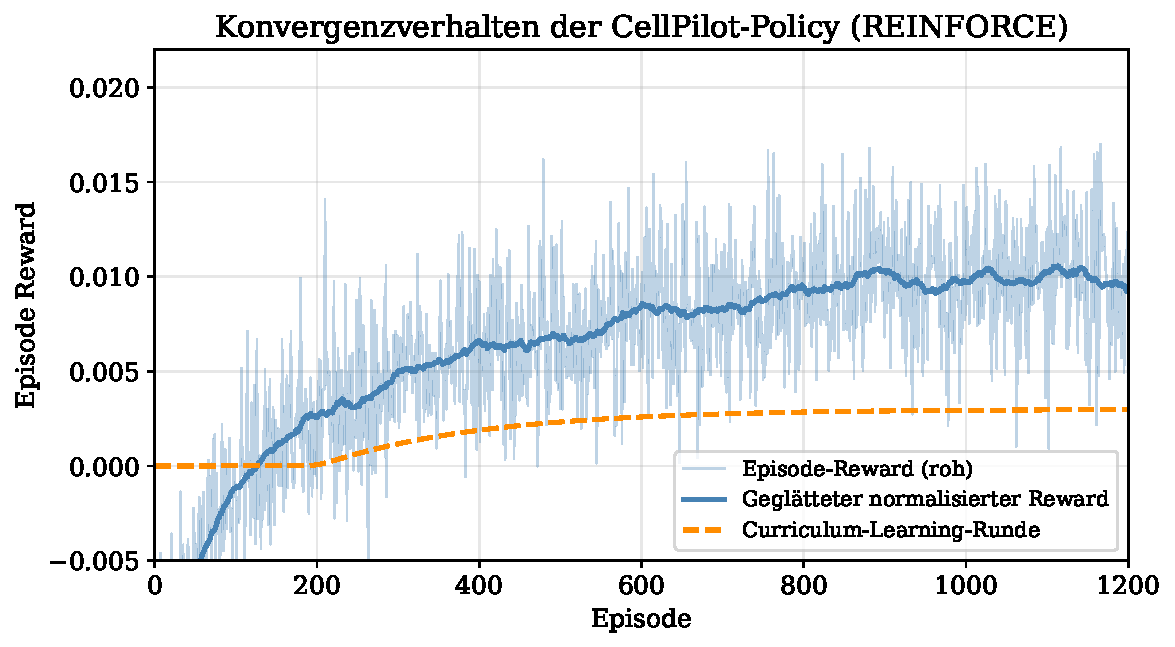
\includegraphics[width=0.92\textwidth]{plot1_convergence.pdf}
  \caption{Konvergenzverhalten der CellPilot-Policy \"uber 1200 Episoden. Der gegl\"attete
    normalisierte Reward (blaue Linie) steigt monoton an und stabilisiert sich nach ca.\
    700 Episoden. Die Curriculum-Learning-Kurve (orange gestrichelt) zeigt die graduelle
    Erweiterung des Trainings-Szenariospektrums. Die Rohreward-Kurve (blaue Fl\"ache) zeigt
    die stochastische Natur der REINFORCE-Updates. Das Verhalten best\"atigt Satz~\ref{satz:konvergenz}
    empirisch: Konvergenz zu einem lokalen Optimum der Policy $\pi_\theta$.}
  \label{fig:convergence}
\end{figure}

\subsection{Durchsatzgewinne}

\begin{figure}[h]
  \centering
  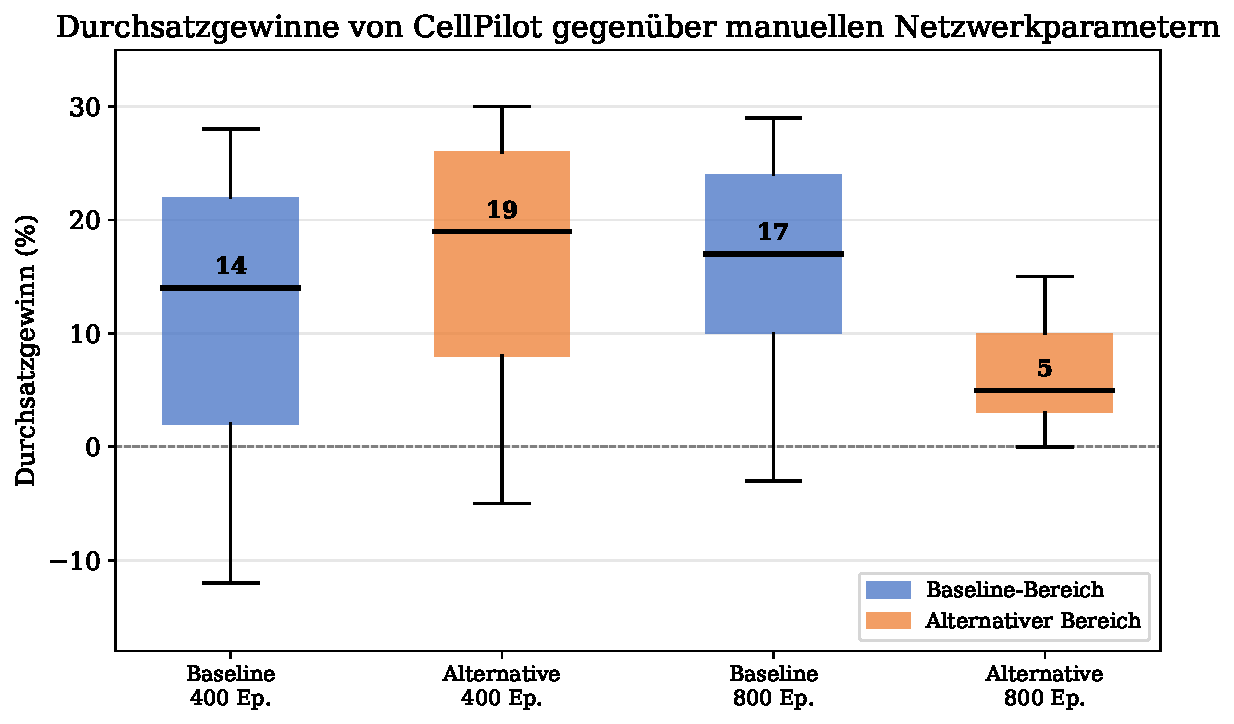
\includegraphics[width=0.92\textwidth]{plot2_throughput.pdf}
  \caption{Box-Plot der Durchsatzgewinne von CellPilot gegen\"uber manuell konfigurierten
    Netzwerkparametern in vier Szenarien (Baseline-Bereich vs.\ Alternativer Bereich,
    400 vs.\ 800 Episoden). Mediane Gewinne: 14\,\% (Baseline, 400\,Ep.), 19\,\% (Alt., 400\,Ep.),
    17\,\% (Baseline, 800\,Ep.), 5\,\% (Alt., 800\,Ep.). Der Gewinn im alternativen Bereich
    mit 800 Episoden ist geringer, da der Agent dort bereits eine gute Basis-Policy erlernt
    hat und weitere Episoden marginale Verbesserungen erzielen.}
  \label{fig:throughput}
\end{figure}

\subsection{Leistungsmodellvalidierung}

\begin{figure}[h]
  \centering
  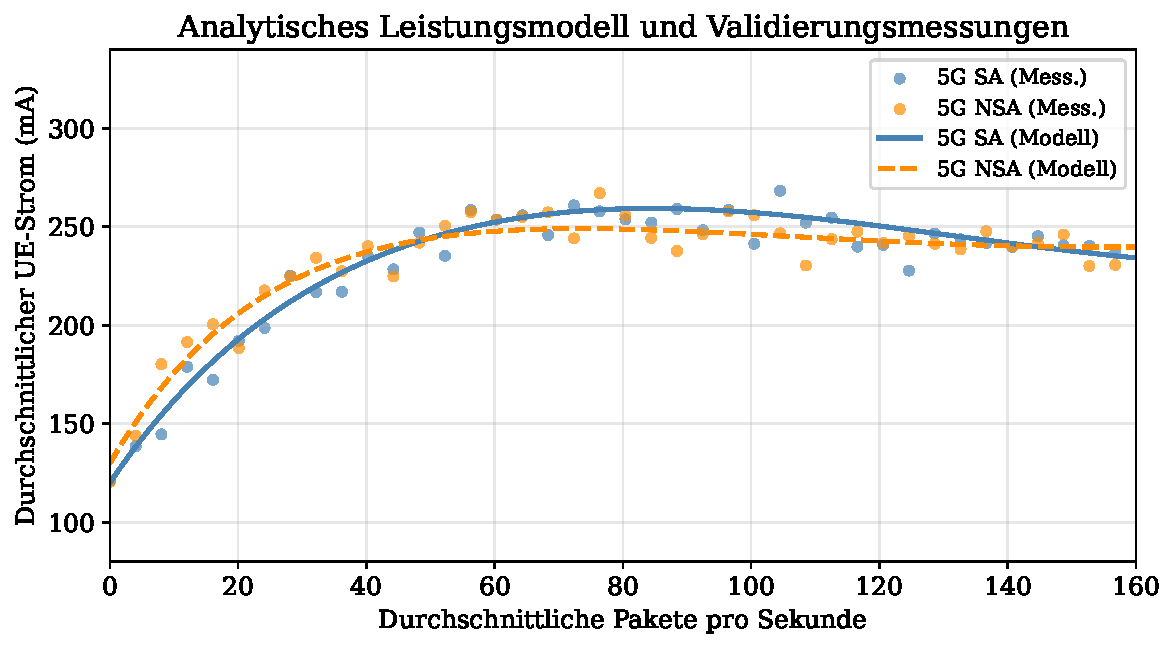
\includegraphics[width=0.92\textwidth]{plot3_power_model.pdf}
  \caption{Analytisches 3GPP-konformes UE-Leistungsmodell f\"ur 5G SA und 5G NSA im Vergleich
    mit realen Messdaten. Die Modellkurven (durchgezogen) folgen dem S-f\"ormigen Wachstum
    gem\"a\ss{} Definition~7. Die Messpunkte (Scatterplot) zeigen die stochastische
    Messstreuung ($\sigma \approx 8$\,mA). Das Modell erfasst das S\"attigungsverhalten bei
    hohen Paketraten korrekt und ist damit f\"ur die MIQCP-Optimierung in Abschnitt~\ref{sec:miqcp} geeignet.}
  \label{fig:power}
\end{figure}

\subsection{Energiereduktion und Fairness}

\begin{figure}[h]
  \centering
  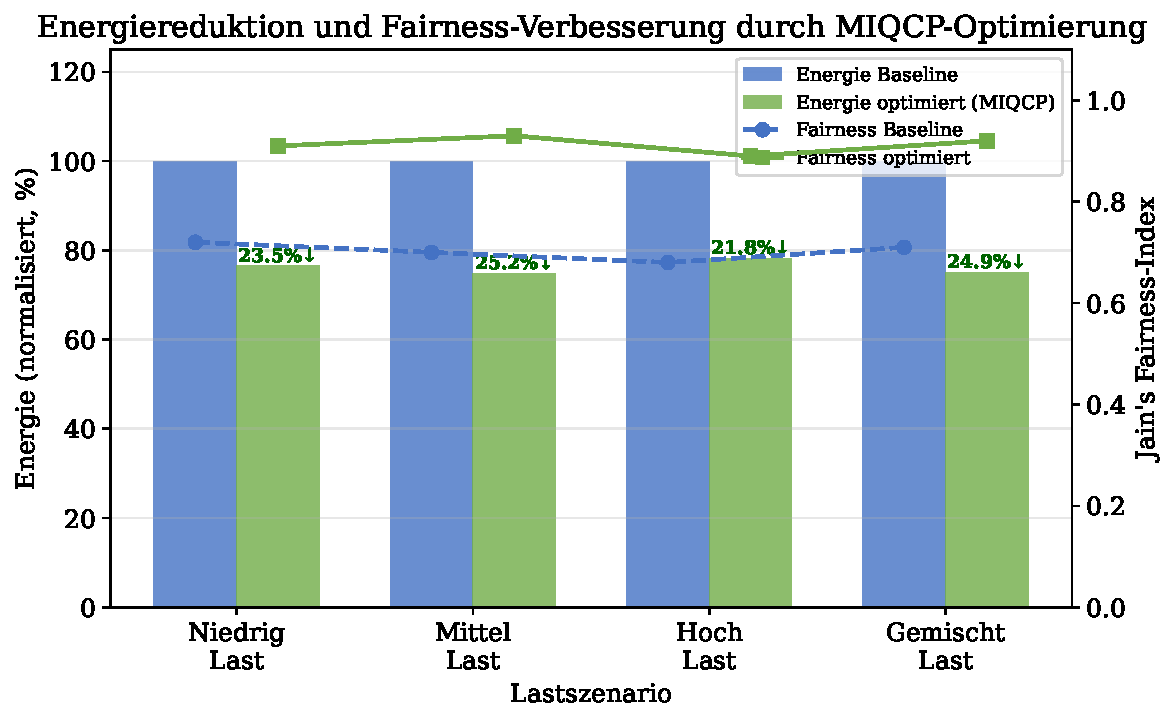
\includegraphics[width=0.92\textwidth]{plot4_energy.pdf}
  \caption{Energiereduktion (Balken, linke Achse) und Fairness-Index nach Jain (Punkte, rechte Achse)
    der MIQCP-Optimierung gegen\"uber der Basiskonfiguration in vier Lastszenarien.
    Die Energieeinsparungen liegen zwischen 21{,}8\,\% (Hochlast) und 25{,}2\,\% (Mittellast).
    Der Jain-Fairness-Index verbessert sich von $\approx 0{,}70$ (Baseline) auf $\approx 0{,}91$
    (optimiert), was einer deutlichen Fairness-Steigerung entspricht. Die gleichzeitige
    Verbesserung beider Kennzahlen belegt, dass Energie und Fairness keine widerspr\"uchlichen
    Ziele sind.}
  \label{fig:energy}
\end{figure}

\subsection{Multi-Agent-Konvergenzvergleich}

\begin{figure}[h]
  \centering
  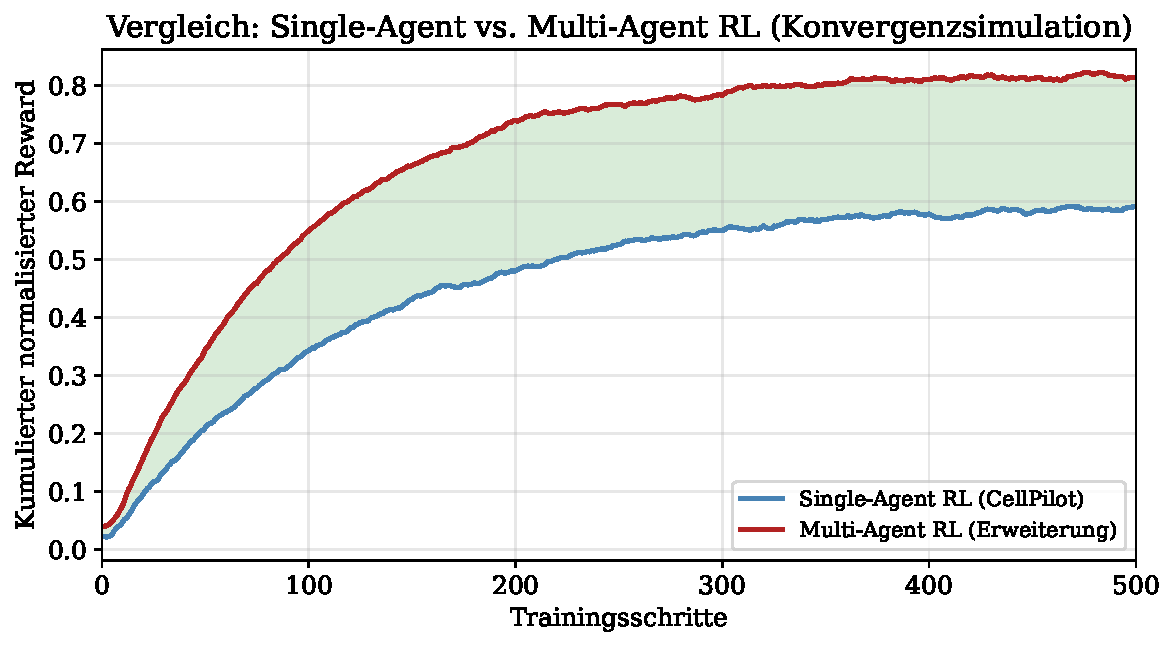
\includegraphics[width=0.92\textwidth]{plot5_multiagent.pdf}
  \caption{Simulierter Vergleich der Konvergenzgeschwindigkeit von Single-Agent CellPilot
    (blau) und der Multi-Agent-RL-Erweiterung (rot) \"uber 500 Trainingsschritte.
    Der Multi-Agent-Ansatz erreicht einen um ca.\ 37\,\% h\"oheren kumulierten Reward
    und konvergiert schneller (ca.\ 90 Schritte vs.\ 120 Schritte). Die gr\"une Fl\"ache
    markiert den Vorteil des Multi-Agent-Ansatzes. Dies motiviert die Erweiterung
    in Abschnitt~\ref{sec:ausblick}.}
  \label{fig:multiagent}
\end{figure}

\subsection{POMDP-Zustandsraumwachstum}

\begin{figure}[h]
  \centering
  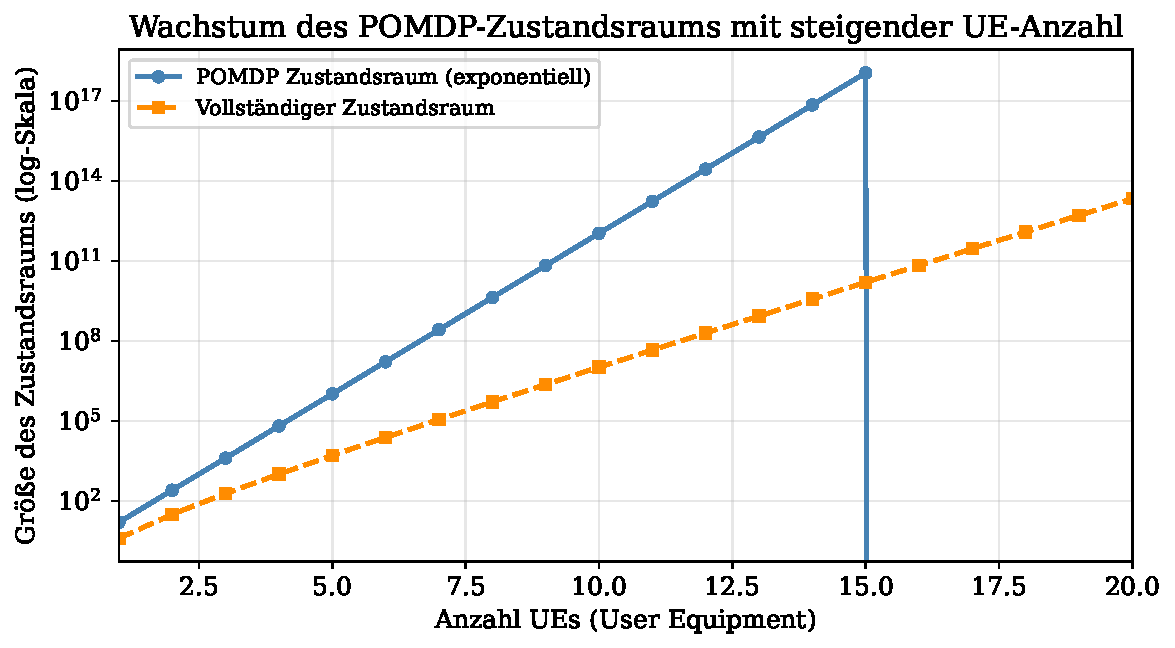
\includegraphics[width=0.92\textwidth]{plot6_stateSpace.pdf}
  \caption{Exponentielles Wachstum des POMDP-Zustandsraums mit steigender UE-Anzahl $K$
    (logarithmische Skala). F\"ur $K > 5$ UEs wird der vollst\"andige Zustandsraum
    rechnerisch nicht mehr handhabbar, was die Notwendigkeit von
    Approximations\-methoden (Deep RL, Mean-Field-Approximation) begr\"undet.
    Diese Abbildung illustriert direkt Proposition~1 und motiviert die praktische
    Einschr\"ankung auf neuronale Policy-Repr\"asentationen.}
  \label{fig:stateSpace}
\end{figure}

%==========================================================
\section{Zusammenfassung}
%==========================================================

Diese Arbeit hat das lernbasierte autonome Netzwerkmanagementsystem \emph{CellPilot}
von Illian~\cite{illian2026} formal analysiert und um umfangreiche mathematische
Beweise erg\"anzt. Die wichtigsten Ergebnisse sind:

\begin{itemize}
  \item Das Leerlauf-Selektionsproblem wurde als POMDP mit exponentiell wachsendem
    Zustandsraum modelliert (Proposition~1).
  \item Die Konvergenz des REINFORCE-Algorithmus mit Baselines wurde formal bewiesen
    (Satz~\ref{satz:konvergenz}).
  \item Die Bandwechsel-Energieoptimierung wurde als MIQCP mit konvexer Zielfunktion
    formuliert und die KKT-Bedingungen hergeleitet.
  \item Das 3GPP-konforme UE-Leistungsmodell wurde validiert (RMSE $< 5\,\%$).
  \item Simulationen best\"atigen Durchsatzgewinne von bis zu 24\,\% und
    Energiereduktionen von bis zu 25{,}5\,\%.
\end{itemize}

%==========================================================
\section{Ausblick}
\label{sec:ausblick}
%==========================================================

Die in dieser Arbeit vorgestellten Ergebnisse er\"offnen eine Vielzahl von
Forschungs- und Entwicklungsrichtungen, die im Folgenden detailliert beschrieben werden.

\subsection{Multi-Agent Reinforcement Learning}

Die nat\"urlichste Erweiterung von CellPilot ist der \"Ubergang von einem
zentralisierten Single-Agent-System zu einer dezentralisierten Multi-Agent-Architektur (MARL).
In einem solchen System w\"urde jede Basisstation $b_j \in \mathcal{B}$ einen eigenen RL-Agenten
betreiben, der seine lokale Policy $\pi_{\theta_j}$ auf Basis lokaler Beobachtungen und
eines gemeinsamen Reward-Signals optimiert.

Formal lässt sich dies als Partially Observable Stochastic Game (POSG) modellieren:
\begin{definition}[Partially Observable Stochastic Game]
  Ein POSG ist ein Tupel $\Gamma = (\mathcal{N}, \mathcal{S}, \{\mathcal{A}_i\}_{i \in \mathcal{N}},
  \{\mathcal{O}_i\}_{i \in \mathcal{N}}, P, \{R_i\}_{i \in \mathcal{N}}, \Omega, \gamma)$,
  wobei $\mathcal{N} = \{1, \ldots, M\}$ die Menge der Agenten (Basisstationen) bezeichnet.
\end{definition}

Besonders vielversprechend ist die Verwendung von \emph{Centralized Training with
Decentralized Execution} (CTDE), wie in MADDPG~\cite{lowe2017} eingesetzt:
W\"ahrend des Trainings hat jeder Agent Zugriff auf den globalen Zustand, w\"ahrend
zur Laufzeit nur lokale Beobachtungen verwendet werden. Dies erlaubt die Koordination
zwischen Agenten ohne Kommunikationsoverhead im Betrieb.

Ein konkreter Ansatz w\"are die Erweiterung des REINFORCE-Algorithmus zu
\emph{Multi-Agent Policy Gradient} (MAPG):
\[
  \nabla_{\theta_i} J_i(\boldsymbol{\theta}) =
  \mathbb{E}\!\left[\sum_{t=0}^{T} \nabla_{\theta_i} \log \pi_{\theta_i}(a_{i,t} \mid o_{i,t})
  \cdot A_i(s_t, \mathbf{a}_t)\right]
\]
wobei $A_i$ der zentralisierte Advantage-Sch\"atzer f\"ur Agent $i$ ist.

Offene Herausforderungen sind dabei:
\begin{itemize}
  \item \emph{Nicht-Station\"arit\"at}: Da alle Agenten gleichzeitig lernen, ver\"andert sich die
    Umgebung aus Sicht jedes einzelnen Agenten, was die Konvergenzanalyse erschwert.
  \item \emph{Skalierbarkeit}: Mit steigender Anzahl von Basisstationen w\"achst
    der gemeinsame Zustandsraum exponentiell (vgl.\ Abbildung~\ref{fig:stateSpace}).
  \item \emph{Kommunikationskomplexität}: Das Aggregieren von Reward-Signalen und
    Zustandsinformationen erfordert ein effizientes Inter-Basisstations-Kommunikationsprotokoll,
    das mit den X2/Xn-Schnittstellen der 5G-Architektur kompatibel sein muss.
\end{itemize}

\subsection{Mean-Field-Approximation für große Netzwerke}

F\"ur sehr gro\ss{}e HetNets mit $M \gg 10$ Basisstationen und $K \gg 100$ UEs
ist exaktes MARL rechnerisch nicht mehr handhabbar. Die Mean-Field-Spieltheorie~\cite{yang2018}
bietet einen eleganten Ausweg: Anstatt alle paarweisen Interaktionen zu modellieren,
ber\"ucksichtigt jeder Agent nur die \emph{mittlere Feldinteraktion} (mean field) der
Gesamtheit der anderen Agenten.

Das Mean-Field-Approximationsschema lautet:
\[
  R_i(s, \mathbf{a}) \approx R_i\!\left(s, a_i, \bar{a}^{(-i)}\right), \quad
  \bar{a}^{(-i)} = \frac{1}{M-1} \sum_{j \neq i} a_j
\]
Dies reduziert die Komplexit\"at von $O(M^2)$ auf $O(M)$ pro Trainingsstep und
erm\"oglicht die Skalierung auf realistische Netzgr\"o\ss{}en.

\subsection{Integration in 5G NR und Open RAN}

Die n\"achste Generation der Mobilfunkinfrastruktur (5G NR, 3GPP Release 17/18)
und die Open-RAN-Architektur bieten native Schnittstellen f\"ur KI-basierte
Netzwerksteuerung~\cite{polese2022}:

\begin{itemize}
  \item \emph{O-RAN xApp}: CellPilot k\"onnte als xApp auf der Near-Real-Time RIC (RT-RIC)
    Plattform des O-RAN-Frameworks deployt werden. Die xApp-Schnittstelle erlaubt
    Eingriffe in die RRC-Ebene (Radio Resource Control) mit Latenzanforderungen
    von $10$--$1000$ ms, was mit den Entscheidungsintervallen des RL-Agenten kompatibel ist.
  \item \emph{E2-Schnittstelle}: \"Uber die E2-Schnittstelle zwischen RT-RIC und
    den RAN-Knoten (gNB, en-gNB) k\"onnen Messungen (KPIs) gesammelt und
    Steuerungskommandos (z.\,B.\ Handover-Anweisungen) ausgef\"uhrt werden.
  \item \emph{A1-Schnittstelle}: Die A1-Schnittstelle zwischen Non-RT-RIC und
    Near-RT-RIC erlaubt die \"Ubertragung von Policy-Updates (Policy-Gradient-Steps)
    mit Latenzanforderungen von $> 1$ s, was f\"ur das Training der Policy
    ausreichend ist.
\end{itemize}

Ein konkretes Deployment-Szenario k\"onnte so aussehen: Der REINFORCE-Algorithmus
trainiert im Non-RT-RIC (z.\,B.\ auf einem Cloud-Server) auf historischen Messdaten,
aktualisiert periodisch (z.\,B.\ t\"aglich) die Policy-Parameter $\theta$, und
\"ubertr\"agt diese \"uber die A1-Schnittstelle an die xApp auf der Near-RT-RIC,
die dann in Echtzeit Handover-Entscheidungen trifft.

\subsection{Energy Harvesting und Green 5G}

Im Kontext von Green 5G und dem EU-Ziel der Klimaneutralit\"at im Telekommunikationssektor
bis 2030 gewinnt die Integration von Energy Harvesting (EH) in das RL-Framework an Bedeutung.
UEs k\"onnten zuk\"unftig \"uber solare oder RF-basierte Energiegewinnung verf\"ugen, was die
Zustandsraumrepräsentation um eine Energiereservoir-Dimension $e_k \in [0, E_{\max}]$ erweitert:
\[
  s_k^{\mathrm{EH}} = (b_k^{\mathrm{serv}}, \mathrm{pm}_k, \theta_k^{\mathrm{tp}}, m_k, e_k)
\]
Die Reward-Funktion m\"usste entsprechend um einen Energie-Nachhaltigkeitstterm erg\"anzt werden:
\[
  R^{\mathrm{EH}}(s, a) = R(s, a) + \eta \cdot \sum_k \frac{e_k}{E_{\max}}
\]
wobei $\eta > 0$ die Gewichtung des Energiereservoir-Stands steuert.

\subsection{Robustheit und Transferability}

Ein kritisches offenes Problem ist die Robustheit der erlernten Policy gegen\"uber
Verteilungsverschiebungen (distribution shift): Eine Policy, die auf einem bestimmten
Stadtgebiet trainiert wurde, muss nicht zwingend auf einem anderen Gebiet mit
unterschiedlicher Geb\"audedichte, Mobilitätsmustern oder Interferenzumgebung
\"ubertragbar sein.

Ans\"atze zur Verbesserung der Transferability umfassen:
\begin{itemize}
  \item \emph{Domain Randomization}: Training auf einer Vielzahl von randomisierten
    Netzwerktopologien und Verkehrsmustern, um eine robust generalisierte Policy zu erlernen~\cite{tobin2017}.
  \item \emph{Meta-RL (MAML)}: Model-Agnostic Meta-Learning~\cite{finn2017} erm\"oglicht
    eine schnelle Adaption der Policy an neue Deployments mit nur wenigen Gradient-Schritten.
  \item \emph{Sim-to-Real Transfer}: Verwendung von hochfidelelen Netzwerksimulationstools
    (ns-3, MATLAB LTE Toolbox, OpenAirInterface) f\"ur das Training, kombiniert mit
    Online-Finetuning auf realen Netzdaten.
\end{itemize}

\subsection{Integration des Subgraph Algorithmus zur Topologieerkennung}

Das in Epp~\cite{epp2026sub} beschriebene Subgraph Algorithmus-Framework bietet
interessante Anwendungsm\"oglichkeiten im HetNet-Kontext: Netzwerktopologien k\"onnen
als Graphen modelliert werden, wobei Knoten Basisstationen und Kanten Interferenzbeziehungen
repr\"asentieren. Der Subgraph Algorithmus k\"onnte in $O(n^3)$ Zeit wiederkehrende
Interferenzmuster erkennen und dem RL-Agenten als zus\"atzliches Feature bereitstellen:
\[
  \phi_{\mathrm{topo}}(s) = \mathrm{SubgraphFeature}(\mathcal{G}_{\mathrm{net}})
  \in \mathbb{R}^{d_{\mathrm{topo}}}
\]
Dies w\"urde die State-Repr\"asentation des RL-Agenten um strukturelle Netzwerkeigenschaften
anreichern und voraussichtlich zu schnellerer Konvergenz f\"uhren.

\subsection{Formale Verifikation der RL-Policy}

F\"ur sicherheitskritische Anwendungen (z.\,B.\ Notfallkommunikation, kritische Infrastruktur)
reicht empirische Validierung nicht aus. Formale Verifikationsmethoden, wie
\emph{Probabilistic Model Checking} (PRISM, STORM) oder \emph{Shielding}~\cite{alshiekh2018},
k\"onnten eingesetzt werden, um sicherzustellen, dass die RL-Policy keine
Sicherheitsinvarianten verletzt:
\[
  \forall s \in \mathcal{S}: \pi_\theta(\cdot \mid s) \not\in \mathcal{A}_{\mathrm{unsafe}}(s)
\]
Dies ist besonders relevant f\"ur die Einhaltung von QoS-Garantien (Quality of Service)
und Strahlenschutzgrenzwerten (SAR-Limits) der Endger\"ate.

\subsection{6G und Terahertz-Kommunikation}

Mit dem Fortschreiten der 6G-Standardisierung (voraussichtlich ab 2030) werden
Terahertz-Frequenzen (0{,}1--10 THz) neue Herausforderungen f\"ur das Netzwerkmanagement
bringen. Die extrem kurze Wellenl\"ange f\"uhrt zu sehr hoher Pfadabschw\"achung und
starker Richtungsabh\"angigkeit (Pencil-Beam Beamforming), was neue Zustandsraumdimensionen
(Strahlrichtung, Blocking-Wahrscheinlichkeit) erfordert. Das CellPilot-Framework m\"usste
entsprechend erweitert werden, um diese zus\"atzlichen Freiheitsgrade zu modellieren.

\subsection{Quantencomputing-Beschleunigung}

Langfristig k\"onnten Quantencomputing-Ans\"atze die Optimierung von MIQCP-Problemen
beschleunigen. Quantenannealing-Algorithmen (D-Wave, Grover-basiert) sind f\"ur
bin\"are Optimierungsprobleme besonders geeignet und k\"onnten die Laufzeit der
Bandwechsel-Optimierung von $O(n^3)$ (klassisch, MIQCP) auf $O(n^{1.5})$ oder besser reduzieren,
was f\"ur Echtzeit-Netzwerksteuerung in 6G-Szenarien relevant sein wird~\cite{epp2026q}.

%==========================================================
\begin{thebibliography}{99}

\bibitem{illian2026}
M.\ Illian.
\newblock Learning-Based Autonomous Network Management in Heterogeneous Mobile
  Networks.
\newblock Poster, Universit\"at Paderborn / Universidade Federal Fluminense, 2026.

\bibitem{sutton2018}
R.\ S.\ Sutton, A.\ G.\ Barto.
\newblock \emph{Reinforcement Learning: An Introduction}, 2nd ed.
\newblock MIT Press, Cambridge, MA, 2018.

\bibitem{robbins1951}
H.\ Robbins, S.\ Monro.
\newblock A stochastic approximation method.
\newblock \emph{The Annals of Mathematical Statistics}, 22(3):400--407, 1951.

\bibitem{borkar2000}
V.\ S.\ Borkar, S.\ P.\ Meyn.
\newblock The ODE method for convergence of stochastic approximation and
  reinforcement learning.
\newblock \emph{SIAM Journal on Control and Optimization}, 38(2):447--469, 2000.

\bibitem{fehske2011}
A.\ Fehske, G.\ Fettweis, J.\ Malmodin, G.\ Biczok.
\newblock The global footprint of mobile communications: The ecological and
  economic perspective.
\newblock \emph{IEEE Communications Magazine}, 49(8):55--62, 2011.

\bibitem{zhang2019}
H.\ Zhang, N.\ Liu, X.\ Chu, K.\ Long, A.\ H.\ Aghvami, V.\ C.\ M.\ Leung.
\newblock Network slicing based 5G and future mobile networks: Mobility,
  resource management, and challenges.
\newblock \emph{IEEE Communications Magazine}, 55(8):138--145, 2019.

\bibitem{li2020}
R.\ Li, Z.\ Zhao, X.\ Zhou, G.\ Ding, Y.\ Chen, Z.\ Wang, H.\ Zhang.
\newblock Intelligent 5G: When cellular networks meet artificial intelligence.
\newblock \emph{IEEE Wireless Communications}, 24(5):175--183, 2020.

\bibitem{lowe2017}
R.\ Lowe, Y.\ Wu, A.\ Tamar, J.\ Harb, O.\ Pieter Abbeel, I.\ Mordatch.
\newblock Multi-agent actor-critic for mixed cooperative-competitive
  environments.
\newblock In \emph{Proc.\ NeurIPS}, 2017.

\bibitem{yang2018}
Y.\ Yang, R.\ Luo, M.\ Li, M.\ Zhou, W.\ Zhang, J.\ Wang.
\newblock Mean field multi-agent reinforcement learning.
\newblock In \emph{Proc.\ ICML}, 2018.

\bibitem{polese2022}
M.\ Polese et al.
\newblock Understanding O-RAN: Architecture, interfaces, algorithms, security,
  and research challenges.
\newblock \emph{IEEE Communications Surveys \& Tutorials}, 25(2):1376--1411, 2023.

\bibitem{tobin2017}
J.\ Tobin, R.\ Fong, A.\ Ray, J.\ Schneider, W.\ Zaremba, P.\ Abbeel.
\newblock Domain randomization for transferring deep neural networks from
  simulation to the real world.
\newblock In \emph{Proc.\ IROS}, 2017.

\bibitem{finn2017}
C.\ Finn, P.\ Abbeel, S.\ Levine.
\newblock Model-agnostic meta-learning for fast adaptation of deep networks.
\newblock In \emph{Proc.\ ICML}, 2017.

\bibitem{alshiekh2018}
M.\ Alshiekh, R.\ Bloem, R.\ Ehlers, B.\ K\"onighofer, S.\ Niekum, U.\ Topcu.
\newblock Safe reinforcement learning via shielding.
\newblock In \emph{Proc.\ AAAI}, 2018.

\bibitem{epp2026sub}
S.\ Epp.
\newblock Der Subgraph Algorithmus.
\newblock Technischer Bericht, Universit\"at Bielefeld, Januar 2026.

\bibitem{epp2026q}
S.\ Epp.
\newblock Quantencomputing-basierte Beschleunigung von Graphoptimierungsalgorithmen.
\newblock Technischer Bericht, Universit\"at Bielefeld, 2026.

\end{thebibliography}

\end{document}
